
%
%  void-input - easy report template for included file
%  EDIT THE LINE ABOVE FOR DOCUMENTATION OF THIS FILE, then delete this line! 
%         

%

% ============================================================
% --- texstudio magic comment: 
% !TEX encoding = UTF-8
% !TeX program = pdflatex
%% !TeX program = xelatex
% !TeX root = "cognome-tesina.tex"
% %  !TeX spellcheck = en_US
% !TeX spellcheck = it_IT


% ====================================================================


\chapter{Task 1}
The execution of this task was quite challenging, requiring special attention in managing the overlap of images and keypoints on numerous different vectors to create a panoramic image. Additionally, I encountered some difficulties in using the cylindricalProj() function, which often generated errors without an apparent cause. However, after a few days of working on the code, I managed to get it to work correctly. To resolve the issues with the includes, I opted to use the ORB algorithm instead of SIFT. Below, you can see the results obtained thanks to the output images.

\begin{figure}[h]
	\centering
        \begin{minipage}{1\textwidth}
        		\centering
		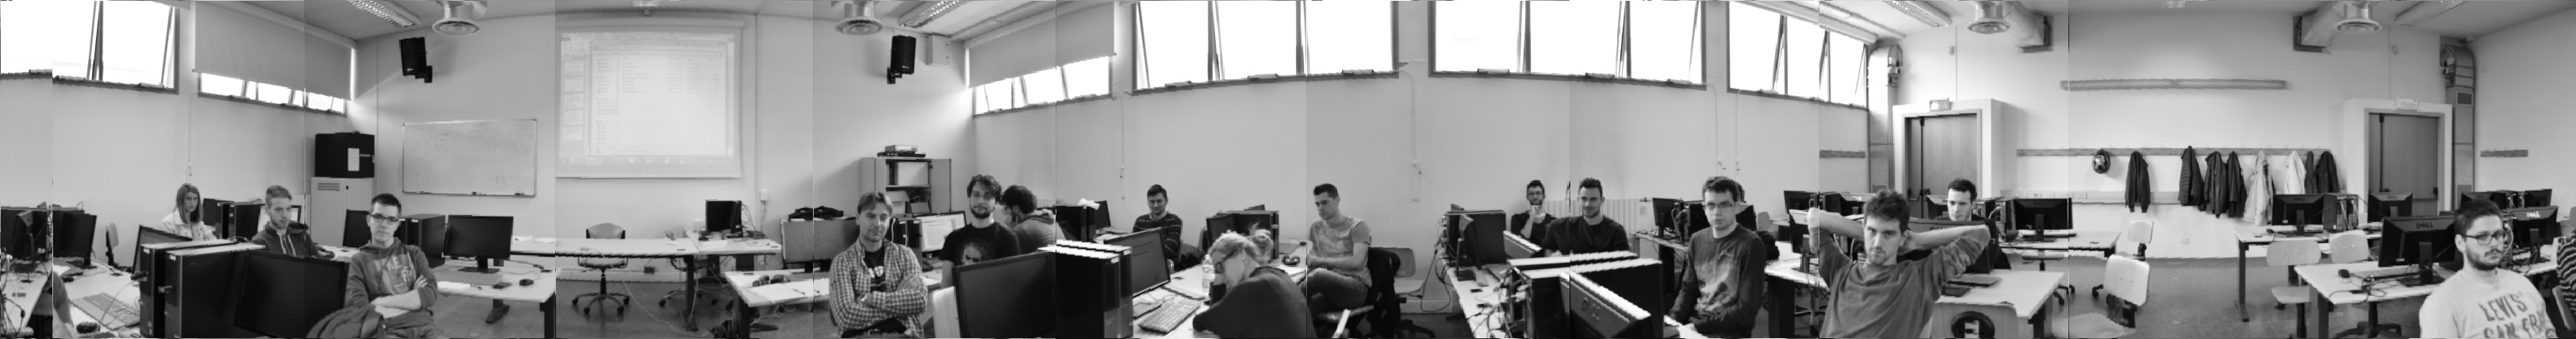
\includegraphics[width=\linewidth]{images/source/1}
		\caption{First image}
		\label{fig:1a}
        \end{minipage}
\end{figure}


\begin{figure}[h]
	\centering
        \begin{minipage}{1\textwidth}
        		\centering
		
\includegraphics[width=\linewidth]{images/source/2}
		\caption{Second image}
		\label{fig:1b}
        \end{minipage}
\end{figure}


\begin{figure}[h]
	\centering
        \begin{minipage}{1\textwidth}
        		\centering
		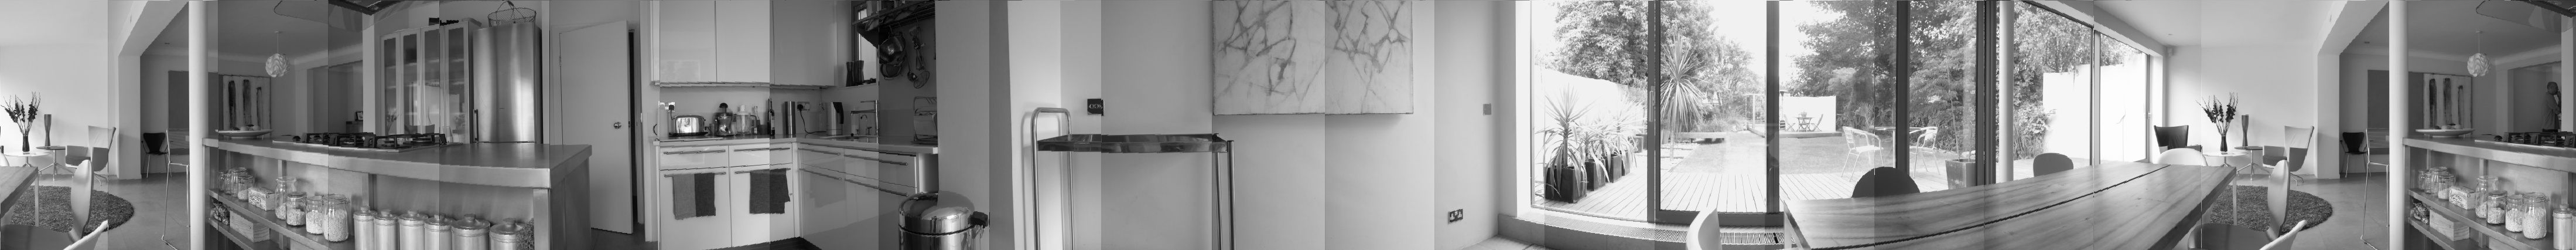
\includegraphics[width=\linewidth]{images/source/3}
		\caption{Third image}
		\label{fig:1c}
        \end{minipage}
\end{figure}

\begin{figure}[h]
	\centering
        \begin{minipage}{1\textwidth}
        		\centering
		
\includegraphics[width=\linewidth]{images/source/4}
		\caption{Fourth image}
		\label{fig:1d}
        \end{minipage}
\end{figure}

\begin{figure}[h]
	\centering
        \begin{minipage}{1\textwidth}
        		\centering
		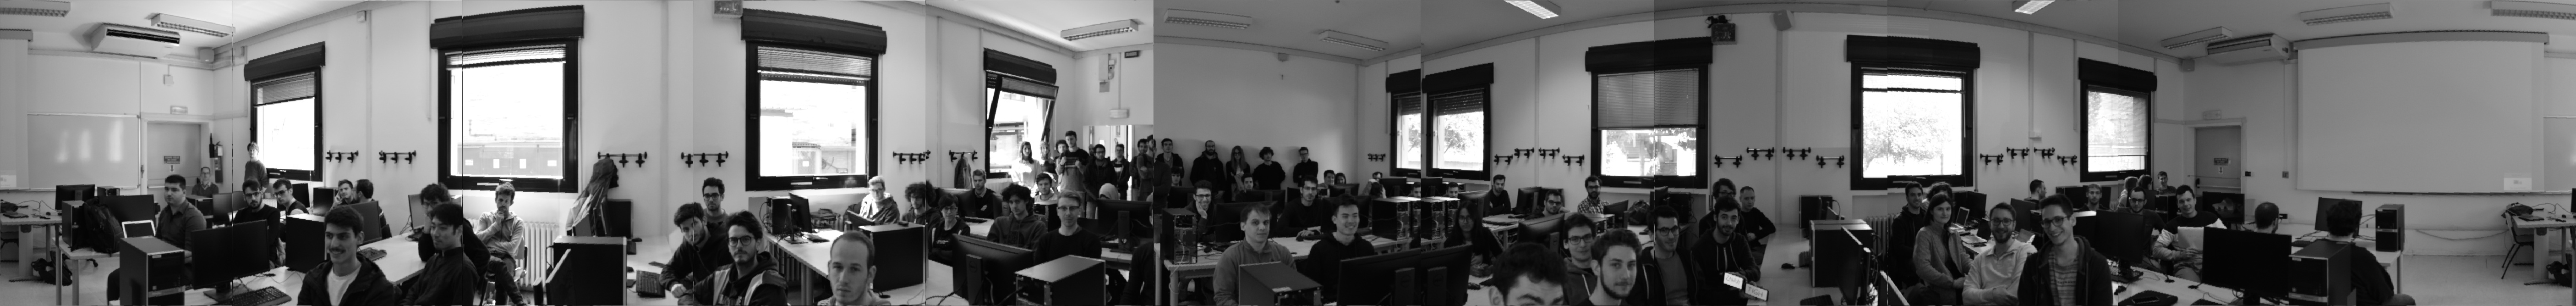
\includegraphics[width=\linewidth]{images/source/5}
		\caption{Fifth image}
		\label{fig:1e}
        \end{minipage}
\end{figure}

% ====================================================================

% ====================================================================
% memo available commands
% ====================================================================
% easyrep: summary of provided macros
%
% \Title{text}     defines the document title 
% \Subtitle{text}  defines the subtitle
% \Author{text}    defines the author string
% \Date{text}      defines a date string
% \printCover      print a cover page using above information
%
% --- text styles
% \tDef{text}      definition (generic) 
% \tDefObj{text}   definition (the ter being defined)
% \tDefTxt{text}   definition (the statement defining the term) 
% \tRemark{text}   remarked text
% \tREMARK{text}   highly remarked text 
% \tLoud{text}     shouted text! 
% \tCode{text}     inline code text
% \tLatin{text}    latin text
% \tForeign{text}  foreign language text 
% \tExample{text}  example 
% \tStandard{text} a recommendation 
% \tQuote{text}    a quoted text 
% \tQuoteFig{text} a quoted text referring to a figure 
% \tConcept{text}  an important concept  
% \tBeginPar{text} highlighted text 
%                  at the beginning of a paragraph 
%
% ---environments
% \begin{quoteStandard} text... \end{quoteStandard}
%    print text to be quoted, e.g. sentences from 
%    a recommendation
%
% \begin{quoteRemark} text... \end{quoteRemark}
%    similar to quoteStandrd, but the text is more marked
%
%  
% --- typo accelerators
% \qmo             opening quotation mark (use \qmo{})
% \qmc             closing quotation mark (use \qmc{})
% \th  emphasises "th"
% \ie  slanted "i.e."
% \eg  slanted "e.g."
% \es  slanteg "ad es."
% \octave   "octave" in \tCode style
% \matlab   "matlab"
% \labview  "labVIEW"
% \latex    "LaTeX" (just the text!)
%
% --- math typo accelerators
% \v{math text}  underlines the math text (useful for vector) 
%
% --- debug commands
% \debugTextStyles        print a table showing text styles
% \debugPrintCharacters   print a table of characters
% \Vispa                  print some text (to fill)  
% \Vispas                 more filling text
% ====================================================================
